\documentclass[a4paper, 12pt]{article}


% Packages
\usepackage[utf8]{inputenc}   % Encoding
\usepackage[T1]{fontenc}      % Font encoding
\usepackage{amsmath, amssymb} % Math packages
\usepackage{graphicx}         % For including images
\usepackage{hyperref}         % For hyperlinks
\usepackage{geometry}         % Page layout
\usepackage{placeins}         % \FloatBarrier
\usepackage{float}            % H

\geometry{a4paper, margin=1in}

% Document information
\title{A1 - Vector Space Models}
\author{Yauheni Zviazdou}
\date{April 19, 2026}

\newtheorem{theorem}{Theorem}

\begin{document}

% Title section
\maketitle

\section{Introduction}

This report details the implementation and evaluation of an experimental Information Retrieval system based on the Vector Space Model (VSM).
The system is designed to rank documents according to their relevance to specific topics using an inverted index.
It supports both English and Czech test collections and experiments with various text preprocessing techniques, term/document weighting schemes, and query expansion methods.

\section{System Architecture Overview}

The system is implemented in Python and operates entirely via the command line.

\subsection{System's Possibilities}

The system supports the following features:
\begin{itemize}
    \item \textbf{Text preprocessing techniques}: lemmatization (using MorphoDiTa tagger \cite{strakova14}), case folding, Part-of-Speech based stopping, and numbers normalization.
    \item \textbf{Document/Query weighting schemes}: (nnn, nnc, ntn, ntc, lnn, lnc, ltn, ltc) for both documents and queries.
    \item \textbf{Query expansion}: Thesaurus-based expansion using synonyms from WordNet
    \begin{itemize}
        \item For English, the system uses the NLTK WordNet \cite{bird-loper-2004-nltk} interface to retrieve synonyms.
        \item For Czech, the system uses the Czech WordNet 1.9 PDT \cite{11858/00-097C-0000-0001-4880-3} to retrieve synonyms.
    \end{itemize}
    \item \textbf{Multiprocessing:} Parallel processing capabilities to speed up processing of large document collections.
\end{itemize}


\subsection{Project structure}

The project codebase is systematically structured into the following core components and configuration files:
\begin{itemize}
    \item \textbf{\texttt{run}}: Serves as the primary executable entry point for the system. It handles command-line argument parsing, environment initialization, and orchestrates the end-to-end retrieval pipeline.
    \item \textbf{\texttt{main.py}}: Encapsulates the core algorithmic logic. It is responsible for constructing the inverted index, applying the selected term-weighting schemes, computing vector space similarities, and ranking documents against the provided queries.
    \item \textbf{\texttt{parser.py}}: Manages the ingestion and preprocessing of structured input data. This includes parsing TREC-formatted topic files and extracting relevant textual content from the SGML-based English and Czech document collections.
    \item \textbf{\texttt{Makefile}}: Automates the project build process, streamlining environment setup and ensuring consistent execution.
    \item \textbf{\texttt{process\_wordnet\_cs.py}}: A specialized utility script that processes the Czech WordNet dataset to generate an optimized, custom JSON dictionary specifically utilized for thesaurus-based query expansion.
    \item \textbf{\texttt{download\_external.sh}}: An automation script designated for acquiring requisite external assets, including the MorphoDiTa tagger models, document and query collections, linguistic databases, and \texttt{trec\_eval} tool.
    \item \textbf{\texttt{requirements.txt}}: Defines the necessary Python runtime dependencies to guarantee a reproducible execution environment.
    \item \textbf{\texttt{README.md}}: Provides documentation, detailing system prerequisites, build instructions, and guidelines for reproducing the experimental runs.
\end{itemize}


\noindent The core operational workflow of the system is driven by two primary functions in \texttt{main.py}:
\begin{itemize}
    \item \textbf{\texttt{init\_index(args)}}: Manages the construction \& saving of the inverted index from the document collection. It also includes built-in functionality to load a pre-computed index from persistent storage to expedite iterative experimentation.
    \item \textbf{\texttt{retrieve\_documents(args)}}: Executes the query evaluation and retrieval phase. It computes the vector space similarities between the formulated queries and the indexed documents to generate a ranked list of relevant results.
\end{itemize}



\section{Building and Execution Instructions}

\subsection{Building}

Download the source code and navigate to the project directory.
Then, run \texttt{make} to build the project.

\textbf{Disclaimer} : the build process primarily involves setting up the Python environment and downloading necessary external resources, rather than traditional compilation.

\subsection{Execution}
The system operates via the command line using the \texttt{run} script.
The script accepts various arguments to specify the input files, output file, and configuration options for the retrieval process.

\subsubsection{Example of use}
\begin{verbatim}
    ./run -q topics.xml -d documents.lst -r run -o sample.res
\end{verbatim}

\newpage 
\subsection{Arguments and Descriptions}


\begin{table}[htbp]
\centering
% \renewcommand{\arraystretch}{1.3}
\begin{tabular}{|l|p{10cm}|}
\hline
\textbf{Argument} & \textbf{Description} \\
\hline
\texttt{-q} & \textbf{Required}. A file including topics in the TREC format (.xml file). \\ \hline
\texttt{-d} & \textbf{Required}. A file including document filenames (.lst file). \\ \hline
\texttt{-r} & \textbf{Required}. A string identifying the experiment run. \\ \hline
\texttt{-o} & \textbf{Required}. The output file for retrieval results (.res file). \\ \hline
\texttt{{-}{-}top\_k} & Number of top documents to retrieve for each query. (Default: 1000) \\ \hline
\texttt{{-}{-}run\_0} & Flag to automatically apply the run-0 (baseline) setup. \\ \hline
\texttt{{-}{-}run\_1} & Flag to automatically apply the run-1 (constrained) setup. \\ \hline
\texttt{{-}{-}run\_2} & Flag to automatically apply the run-2 (unconstrained) setup. \\ \hline
\texttt{{-}{-}lemmatization} & Flag to lemmatize tokens using the MorphoDiTa tagger. \\ \hline
\texttt{{-}{-}case\_folding} & Flag to apply case folding (lowercasing) to tokens. \\ \hline
\texttt{{-}{-}pos\_stopping} & Flag to apply Part-of-Speech based stopping. \\ \hline
\texttt{{-}{-}number\_normalization} & Flag to normalize all numeric digits to a standard \texttt{<NUM>} token. \\ \hline
\texttt{{-}{-}doc\_weights} & Weighting scheme for document terms. Possible values: (\texttt{nnn}, \texttt{nnc}, \texttt{ntn}, \texttt{ntc}, \texttt{lnn}, \texttt{lnc}, \texttt{ltn}, \texttt{ltc}). \\ \hline
\texttt{{-}{-}query\_weights} & Weighting scheme for query terms. Possible values: (\texttt{nnn}, \texttt{nnc}, \texttt{ntn}, \texttt{ntc}, \texttt{lnn}, \texttt{lnc}, \texttt{ltn}, \texttt{ltc}). \\ \hline
\texttt{{-}{-}use\_query\_description} & Flag to expand the query using the topic \texttt{<desc>} and \texttt{<narr>} fields. \\ \hline
\texttt{{-}{-}thesaurus\_n} & Number of synonyms to retrieve from the WordNet/custom thesaurus. \\ \hline
\texttt{{-}{-}cpu\_n} & Number of CPU cores to allocate for parallel processing (-1 for all cores). \\ \hline
\texttt{{-}{-}save\_index} & Flag to save the constructed inverted index to disk for future runs. \\ \hline
\texttt{{-}{-}load\_index} & Flag to load a pre-computed inverted index from disk instead of constructing it from the document collection. \\
\hline
\end{tabular}
\caption{Command-line arguments and descriptions for \texttt{run}}
\label{tab:main_args}
\end{table}

\newpage

\section{Experiments Setups}

\subsection{Run-0 Setup (Baseline) }

The run-0 setup serves as a baseline for evaluating the performance of the retrieval system.

Settings for run-0:
\begin{itemize}
    \item \textbf{tokenization}: whitespace+punctuation
    \item \textbf{class equivalence}: no
    \item \textbf{removing stopwords}: no
    \item \textbf{query construction}: all words from ”title”
    \item \textbf{term weighting}: natural
    \item \textbf{document frequency weighting}: none
    \item \textbf{vector normalization}: cosine
    \item \textbf{similarity measurement}: cosine
    \item \textbf{relevance feedback}: none
    \item \textbf{query expansion}: none
\end{itemize}

This setup can be executed using the following command:
\begin{verbatim}
    ./run -q topics.xml -d documents.lst -r run-0 -o run-0.res --run-0
\end{verbatim}

\subsection{Run-1 Setup (Constrained)}

The run-1 setup applies a series of preprocessing and weighting techniques to enhance the retrieval performance while adhering to the constraints specified in the assignment.

Settings for run-1:
\begin{itemize}
    \item \textbf{tokenization}: whitespace+punctuation
    \item \textbf{class equivalence}: case folding, lemmatization (using MorphoDiTa tagger).
    \item \textbf{removing stopwords}: None.
    \item \textbf{query construction}: Topic titles only.
    \item \textbf{term weighting}: Logarithmic (\texttt{l}) for both documents and queries.
    \item \textbf{document frequency weighting}: IDF (\texttt{t}) for documents; None (\texttt{n}) for queries.
    \item \textbf{vector normalization}: None (\texttt{n}) for documents; Cosine normalization (\texttt{c}) for queries.
    \item \textbf{similarity measurement}: Cosine similarity.
    \item \textbf{relevance feedback}: None.
    \item \textbf{query expansion}: Thesaurus-based expansion (with scaling 0.2). 
\end{itemize}

This setup can be executed using the following command:
\begin{verbatim}
    ./run -q topics.xml -d documents.lst -r run-1 -o run-1.res --run-1
\end{verbatim}


\section{Results and Evolution of Results}

We conducted a series of experiments to evaluate the performance of the retrieval system under different configurations.
The results are presented in terms of Mean Average Precision (MAP) for both English and Czech collections.
Goal of the experiments was to iteratively improve the retrieval performance by applying various techniques.

\subsection{Initial setup (Run-0)}

The initial run-0 setup, which serves as a baseline, achieved MAP scores of 0.0411 for the English collection and 0.0596 for the Czech collection.

\begin{table}[H]
    \centering
    \begin{tabular}[t]{p{3cm}cc} 
        \hline
        \textbf{Setup} & \textbf{English} (map) & \textbf{Czech} (map) \\ 
        \hline
        \texttt{Run-0} & 0.0411 & 0.0596 \\
        \hline
    \end{tabular}
    \caption{Initial setup (Run-0) results.}
    \label{tab:run0_results}
\end{table}

\subsection{Documents and Queries weighting schemes}

To optimize the Vector Space Model (VSM), we experimented with various term-weighting strategies.
A complete weighting scheme consists of two parts: the document weighting and the query weighting. 

Each weighting scheme is defined by a three-letter code representing three independent components: \textbf{Term Frequency}, \textbf{Document Frequency}, and \textbf{Normalization}.
For this experiment, we implemented 2 specific possibilities for each component:

\begin{enumerate}
    \item \textbf{Term Frequency Weighting:}
    \begin{itemize}
        \item \texttt{n} (natural): The raw term frequency is used without modification.
        \item \texttt{l} (logarithmic): The term frequency is dampened using a base-10 logarithm to reduce the disproportionate impact of highly frequent terms. 
    \end{itemize}

    \item \textbf{Document Frequency Weighting:}
    \begin{itemize}
        \item \texttt{n} (none): No global weighting is applied. The multiplier is simply $1$.
        \item \texttt{t} (inverse document frequency): Rare terms are rewarded, and common terms are penalized using IDF.
    \end{itemize}

    \item \textbf{Vector Normalization:}
    \begin{itemize}
        \item \texttt{n} (none): No normalization is applied to the final vector.
        \item \texttt{c} (cosine): The vector is scaled by its Euclidean length.
    \end{itemize}
\end{enumerate}

There is 64 possible combinations of weighting schemes for documents and queries, which are represented by three-letter codes for documents and queries, respectively.

We conducted a grid search across all 64 possible combinations. The Mean Average Precision (MAP) results for both the English and Czech test collections are summarized in Table~\ref{tab:weighting_schemes}.


\begin{table}[H]
    \centering
    \begin{tabular}[t]{p{3cm}cc} 
        \hline
        \textbf{Scheme} & \textbf{English} & \textbf{Czech} \\ 
        \hline
        \texttt{nnn.nnn} & 0.0765 & 0.0366 \\
        \texttt{nnn.nnc} & 0.0765 & 0.0366 \\
        \texttt{nnn.ntn} & 0.1171 & 0.0595 \\
        \texttt{nnn.ntc} & 0.1171 & 0.0595 \\
        \texttt{nnn.lnn} & 0.0765 & 0.0366 \\
        \texttt{nnn.lnc} & 0.0765 & 0.0366 \\
        \texttt{nnn.ltn} & 0.1171 & 0.0595 \\
        \texttt{nnn.ltc} & 0.1171 & 0.0595 \\
        \texttt{nnc.nnn} & 0.0415 & 0.0594 \\
        \texttt{nnc.nnc} & 0.0415 & 0.0594 \\
        \texttt{nnc.ntn} & 0.0827 & 0.0939 \\
        \texttt{nnc.ntc} & 0.0827 & 0.0939 \\
        \texttt{nnc.lnn} & 0.0415 & 0.0594 \\
        \texttt{nnc.lnc} & 0.0415 & 0.0594 \\
        \texttt{nnc.ltn} & 0.0827 & 0.0939 \\
        \texttt{nnc.ltc} & 0.0827 & 0.0939 \\
        \texttt{ntn.nnn} & 0.1171 & 0.0595 \\
        \texttt{ntn.nnc} & 0.1171 & 0.0595 \\
        \texttt{ntn.ntn} & 0.1481 & 0.0913 \\
        \texttt{ntn.ntc} & 0.1481 & 0.0913 \\
        \texttt{ntn.lnn} & 0.1171 & 0.0595 \\
        \texttt{ntn.lnc} & 0.1171 & 0.0595 \\
        \texttt{ntn.ltn} & 0.1481 & 0.0913 \\
        \texttt{ntn.ltc} & 0.1481 & 0.0913 \\
        \texttt{ntc.nnn} & 0.0953 & 0.0869 \\
        \texttt{ntc.nnc} & 0.0953 & 0.0869 \\
        \texttt{ntc.ntn} & 0.1117 & 0.1292 \\
        \texttt{ntc.ntc} & 0.1117 & 0.1292 \\
        \texttt{ntc.lnn} & 0.0953 & 0.0869 \\
        \texttt{ntc.lnc} & 0.0953 & 0.0869 \\
        \texttt{ntc.ltn} & 0.1117 & 0.1292 \\
        \texttt{ntc.ltc} & 0.1117 & 0.1292 \\
        \hline
    \end{tabular}%
    \hfill%
    \begin{tabular}[t]{p{3cm}cc} 
        \hline
        \textbf{Scheme} & \textbf{English} & \textbf{Czech} \\ 
        \hline
        \texttt{lnn.nnn} & 0.1879          & 0.1278 \\
        \texttt{lnn.nnc} & 0.1879          & 0.1278 \\
        \texttt{lnn.ntn} & \textbf{0.2239} & \textbf{0.1626} \\
        \texttt{lnn.ntc} & \textbf{0.2239} & \textbf{0.1626} \\
        \texttt{lnn.lnn} & 0.1879          & 0.1278 \\
        \texttt{lnn.lnc} & 0.1879          & 0.1278 \\
        \texttt{lnn.ltn} & \textbf{0.2239} & \textbf{0.1626} \\
        \texttt{lnn.ltc} & \textbf{0.2239} & \textbf{0.1626} \\
        \texttt{lnc.nnn} & 0.0492          & 0.0692 \\
        \texttt{lnc.nnc} & 0.0492          & 0.0692 \\
        \texttt{lnc.ntn} & 0.0910          & 0.1087 \\
        \texttt{lnc.ntc} & 0.0910          & 0.1087 \\
        \texttt{lnc.lnn} & 0.0492          & 0.0692 \\
        \texttt{lnc.lnc} & 0.0492          & 0.0692 \\
        \texttt{lnc.ltn} & 0.0910          & 0.1087 \\
        \texttt{lnc.ltc} & 0.0910          & 0.1087 \\
        \texttt{ltn.nnn} & \textbf{0.2239} & \textbf{0.1626} \\
        \texttt{ltn.nnc} & \textbf{0.2239} & \textbf{0.1626} \\
        \texttt{ltn.ntn} & 0.1968          & 0.1556 \\
        \texttt{ltn.ntc} & 0.1968          & 0.1556 \\
        \texttt{ltn.lnn} & \textbf{0.2239} & \textbf{0.1626} \\
        \texttt{ltn.lnc} & \textbf{0.2239} & \textbf{0.1626} \\
        \texttt{ltn.ltn} & 0.1968          & 0.1556 \\
        \texttt{ltn.ltc} & 0.1968          & 0.1556 \\
        \texttt{ltc.nnn} & 0.0848          & 0.0975 \\
        \texttt{ltc.nnc} & 0.0848          & 0.0975 \\
        \texttt{ltc.ntn} & 0.1006          & 0.1178 \\
        \texttt{ltc.ntc} & 0.1006          & 0.1178 \\
        \texttt{ltc.lnn} & 0.0848          & 0.0975 \\
        \texttt{ltc.lnc} & 0.0848          & 0.0975 \\
        \texttt{ltc.ltn} & 0.1006          & 0.1178 \\
        \texttt{ltc.ltc} & 0.1006          & 0.1178 \\
        \hline
    \end{tabular}
    
    % \vspace{0.5cm} % Adds a little breathing room before the caption
    \caption{Weighting schemes for documents and queries. Results are shown in terms of MAP.}
    \label{tab:weighting_schemes}
\end{table}

\FloatBarrier

Scheme \texttt{ltn.lnc} was the best performing scheme for both English and Czech collections, achieving the highest MAP scores of 0.2239 and 0.1626, respectively.
This scheme was chosen for the run-1 setup.

\newpage

\subsection{Lemmatization + POS-based stopping}

Next step was to apply lemmatization, POS-based stopping and their combination.
The results are shown in the Table~\ref{tab:lemmatization_pos_stopping}.

\begin{table}[h]
    \centering
    \begin{tabular}[t]{lcc} 
        \hline
        \textbf{Approach} & \textbf{English} (map) & \textbf{Czech} (map) \\ 
        \hline
         pos\_stopping & 0.1865 & 0.1624 \\
         lemmatization & \textbf{0.2527} & \textbf{0.3224} \\
         lemmatization + pos\_stopping & 0.2498 & 0.3177 \\
        \hline
    \end{tabular}
    \caption{Lemmatization and POS-based stopping}
    \label{tab:lemmatization_pos_stopping}
\end{table}

Lemmatization significantly improved the MAP scores for both English and Czech collections, increasing them to 0.2527 and 0.3224, respectively.
POS-based stopping alone did not improve the performance, probably POS-based stopping was too strict.

\subsection{Query expansion}

Next step was to apply thesaurus-based query expansion using synonyms from WordNet.
We retrieved all synonyms and added weights of them to the query with additional scaling factor.
To select the best scaling factor, we experimented with different values and found that 0.2 was the best performing one for both English and Czech collections, Fig.~\ref{fig:query_expansion}.

\begin{figure}[H]
    \centering
    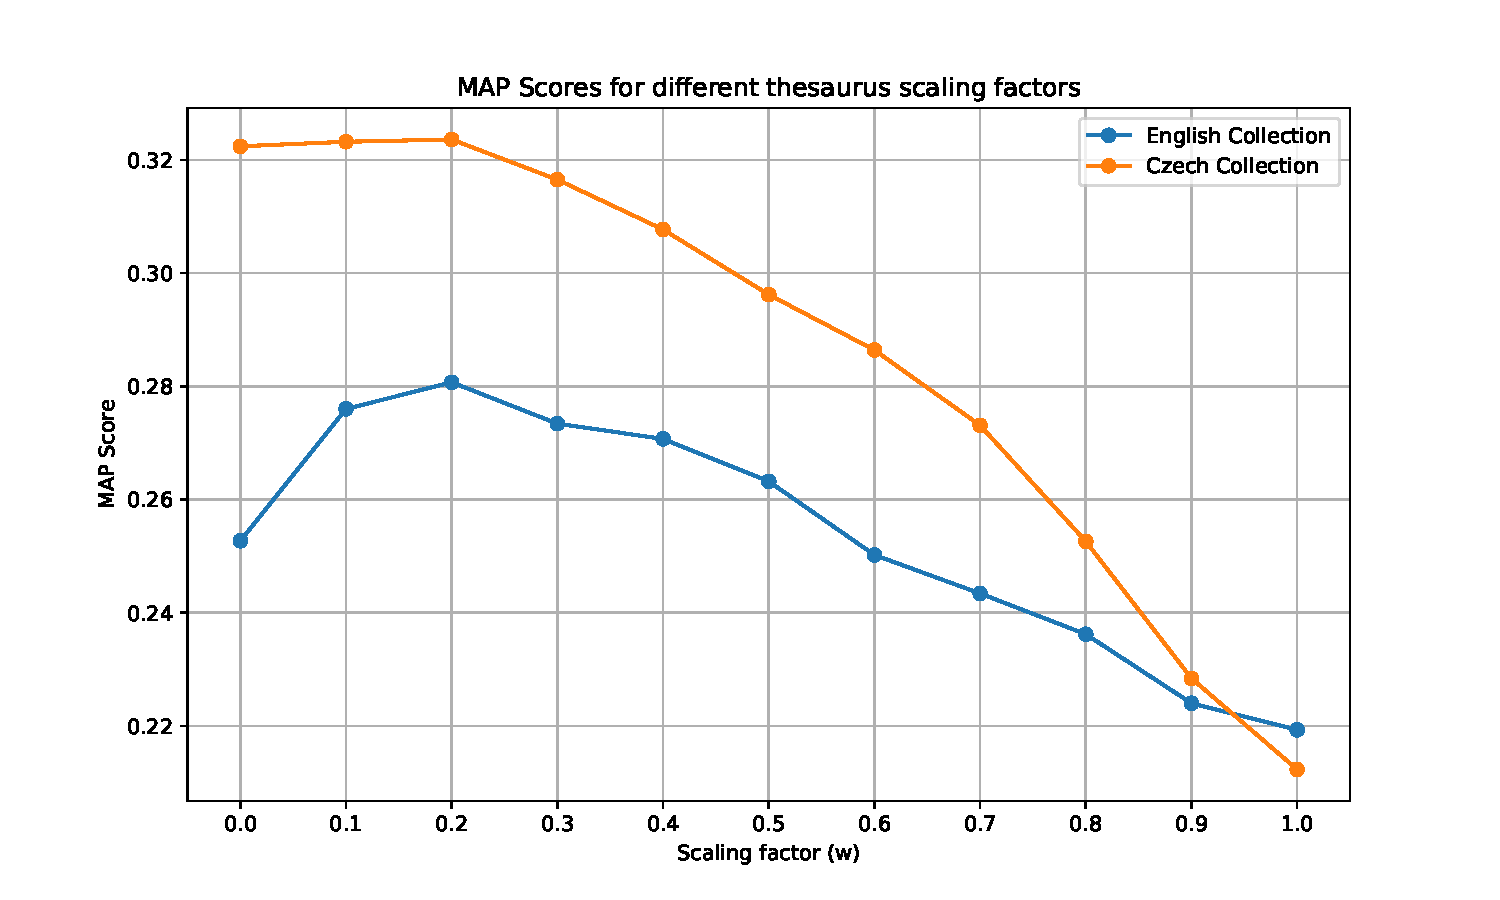
\includegraphics[width=0.8\textwidth]{figures/thesaurus_plot.pdf}
    \caption{Thesaurus-based query expansion using synonyms from WordNet.}
    \label{fig:query_expansion}
\end{figure}

Detailed data of experiment are shown in the Table~\ref{tab:query_expansion}.

\begin{table}[h]
    \centering
    \begin{tabular}[t]{lcc} 
        \hline
        \textbf{Scaling Factor} & \textbf{English} (map) & \textbf{Czech} (map) \\ 
        \hline
        0.0 & 0.2527 & 0.3224 \\
        0.1 & 0.2760 & 0.3232 \\
        0.2 & \textbf{0.2807} & \textbf{0.3236} \\
        0.3 & 0.2734 & 0.3165 \\
        0.4 & 0.2707 & 0.3077 \\
        0.5 & 0.2632 & 0.2962 \\
        0.6 & 0.2502 & 0.2864 \\
        0.7 & 0.2434 & 0.2731 \\
        0.8 & 0.2362 & 0.2526 \\
        0.9 & 0.2240 & 0.2284 \\
        1.0 & 0.2193 & 0.2123 \\
        \hline
    \end{tabular}
    \caption{Thesaurus-based query expansion}
    \label{tab:query_expansion}
\end{table}

\FloatBarrier

\subsection{Final Results}

Table~\ref{tab:final_results} summarizes the overall performance leap from the initial baseline (Run-0) to the fully optimized constrained system (Run-1).

\begin{table}[h]
    \centering
    \begin{tabular}[t]{lcc} 
        \hline
        \textbf{Approach} & \textbf{English} (map) & \textbf{Czech} (map) \\ 
        \hline
         Run-0 (Baseline) & 0.0411 & 0.0596\\
         Run-1 (Constrained) & 0.2807 & 0.3236 \\
        \hline
    \end{tabular}
    \caption{Final Results}
    \label{tab:final_results}
\end{table}

By systematically integrating the \texttt{ltn.lnc} weighting scheme, MorphoDiTa-based lemmatization, and appropriately scaled thesaurus expansion, the system achieved big improvements in retrieval performance for both English and Czech collections.

Run-1 is 6.8 times better than Run-0 for English collection and 5.4 times better for Czech collection in terms of MAP.

\section{Summary}
The implemented Information Retrieval system based on the Vector Space Model demonstrated significant improvements in retrieval performance through the application of lemmatization and thesaurus-based query expansion.

Lemmatization alone resulted in a substantial increase in MAP scores for both English and Czech collections, while the addition of POS-based stopping did not yield further benefits.

Thesaurus-based query expansion, when applied with an optimal scaling factor of 0.2, significantly improved the retrieval performance, further enhancing the MAP scores for both collections.

The final run-1 setup, which incorporated lemmatization and thesaurus-based query expansion, achieved the highest MAP scores 0.2807 (English) and 0.3236 (Czech).

% References
\bibliographystyle{plain}
\bibliography{references}

\end{document}
